\PassOptionsToPackage{unicode}{hyperref}
\PassOptionsToPackage{hyphens}{url}
%
\documentclass[12pt]{article}
\usepackage{amsmath,amssymb}
\usepackage{lmodern}
\usepackage{iftex}
\ifPDFTeX
  \usepackage[T1]{fontenc}
  \usepackage[utf8]{inputenc}
  \usepackage{textcomp} % provide euro and other symbols
\else % if luatex or xetex
  \usepackage{unicode-math}
  \defaultfontfeatures{Scale=MatchLowercase}
  \defaultfontfeatures[\rmfamily]{Ligatures=TeX,Scale=1}
\fi
\IfFileExists{upquote.sty}{\usepackage{upquote}}{}
\IfFileExists{microtype.sty}{\usepackage[]{microtype}}{}
\usepackage{xcolor}
\setlength{\emergencystretch}{3em} % prevent overfull lines
\providecommand{\tightlist}{%
  \setlength{\itemsep}{0pt}\setlength{\parskip}{0pt}}
\setcounter{secnumdepth}{-\maxdimen} % remove section numbering
\ifLuaTeX
  \usepackage{selnolig}  % disable illegal ligatures
\fi
\IfFileExists{bookmark.sty}{\usepackage{bookmark}}{\usepackage{hyperref}}
\IfFileExists{xurl.sty}{\usepackage{xurl}}{} % add URL line breaks if available
\urlstyle{same} % disable monospaced font for URLs
\hypersetup{
  hidelinks,
  pdfcreator={LaTeX via pandoc}}

\author{}
\date{}

\begin{document}

\textbf{Genome Wide Association Study (GWAS)}

\textbf{Student Name:} Prit Desai\\
\textbf{UTA ID:} 1002170533\\
\textbf{Course:} CSE 5370 - Bioinformatics\\
\textbf{Assignment:} Homework 1

\section*{1.2 Fisher's Exact Test}

The null hypothesis (H₀) for the Fisher's Exact Test states that there is no association between the presence of the C-allele at a given SNP and the complex genetic trait being studied. In other words, the odds ratio between case and control groups for the C-allele is equal to 1. Rejecting this null hypothesis suggests that the SNP may be associated with the trait.

\textbf{Choice of Alternative Hypothesis:} The test uses the alternative="two-sided" option because the analysis aims to detect any association between SNP presence and the trait, whether positive or negative. This ensures that SNPs with either increased or decreased associations are identified.

\textbf{Number of Significant SNPs:}
\begin{itemize}
  \item \textbf{Significant SNPs under Original Threshold (5 × 10⁻⁸):} 11
  \item \textbf{Significant SNPs under Bonferroni Correction (5 × 10⁻¹¹):} 3
\end{itemize}

\section*{1.3 Bonferroni Correction}

The Bonferroni correction addresses the multiple hypothesis testing issue by adjusting the significance threshold. Since 1000 SNPs are tested, the corrected p-value threshold is:

\[
\frac{5 \times 10^{-8}}{1000} = 5 \times 10^{-11}
\]

This correction reduces the likelihood of Type I errors but increases the chance of Type II errors, making the test more conservative and resulting in fewer significant SNPs compared to the original threshold.

\section*{1.4 Manhattan Plot Interpretation}

The Manhattan plot visualizes the -log₁₀(p-values) of each SNP locus. Higher points indicate stronger evidence against the null hypothesis.

\textbf{Key Observations:}
\begin{itemize}
  \item \textbf{Red dashed line:} Original significance threshold (5 × 10⁻⁸)
  \item \textbf{Blue dashed line:} Bonferroni-corrected threshold (5 × 10⁻¹¹)
  \item \textbf{Points above the lines:} Statistically significant SNPs
  \item A cluster of significant SNPs between loci 450 and 470 indicates a potential genomic region associated with the trait.
\end{itemize}

\begin{figure}[h!]
\centering
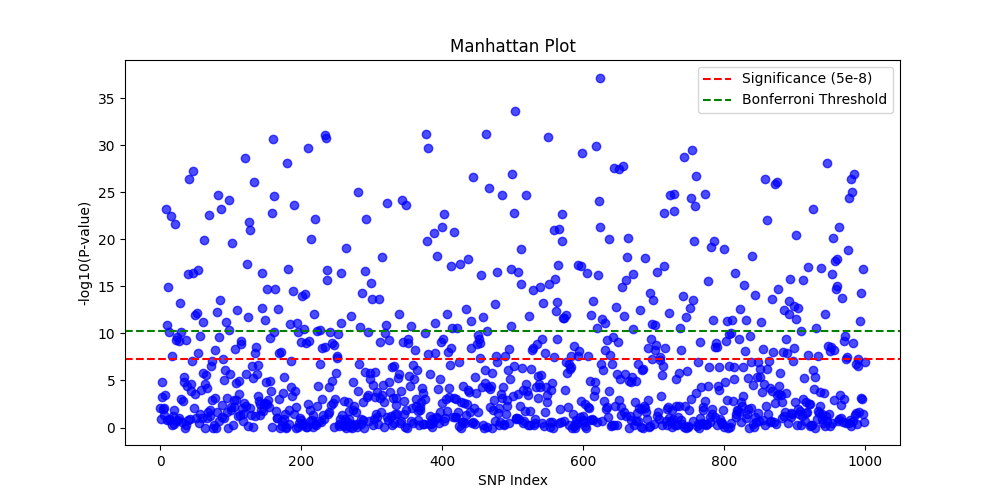
\includegraphics[width=0.8\textwidth]{manhattan_plot.png}
\caption{Manhattan Plot for GWAS showing the SNPs with their p-values. The red and blue dashed lines represent the original and Bonferroni-corrected significance thresholds, respectively.}
\end{figure}

\section*{Files Included in Submission}
\begin{itemize}
  \item 1002170533.csv: Generated dataset
  \item results.csv: SNP names, p-values, and significance indicators
  \item manhattan\_plot.png: Visualization of GWAS results
  \item GWAS\_Writeup.pdf: This document
  \item readme.txt: Instructions to run the code
  \item Source Code:
    \begin{itemize}
      \item datasetGenerator.py: Dataset generation
      \item HW1.py: GWAS analysis (Fisher's test and Manhattan plot)
    \end{itemize}
\end{itemize}

\section*{Instructions to Run Code}
\begin{enumerate}
  \item Install Python (version ≥ 3.8) and required libraries: numpy, scipy, matplotlib.
  \item Activate the virtual environment:
    \begin{verbatim}
    .\venv\Scripts\Activate
    \end{verbatim}
  \item Run the dataset generator:
    \begin{verbatim}
    python datasetGenerator.py --ID 1002170533
    \end{verbatim}
  \item Run the analysis script:
    \begin{verbatim}
    python HW1.py
    \end{verbatim}
  \item Outputs:
    \begin{itemize}
      \item results.csv: Contains p-values and significance flags
      \item manhattan\_plot.png: Displayed and saved automatically
    \end{itemize}
\end{enumerate}

\section*{Difficulty \& Time Spent}
\begin{itemize}
  \item \textbf{Estimated Time:} 10 hours
  \item \textbf{Challenges:} Understanding the Bonferroni correction and interpreting the plot required extra time.
\end{itemize}


\end{document}
